\documentclass[a4paper,twoside,french,10pt]{VcCours}

\newcommand{\dt}{\text{d}t}
\newcommand{\dx}{\text{d}x}
\newcommand{\Sum}[2]{\sum_{#1}^{#2}}
\newcommand{\enc}[1]{\begin{center}\fbox{#1}\end{center}}

\begin{document}
\Titre{PSI}{Promotion 2021--2022}{Mathématiques}{Devoir non surveillé n\degres5}

\begin{center}
\large\bf
Correction
\end{center}
\separationTitre


\section*{Exercice 1}
\begin{enumerate}
  \item Soit $n \in \mathbb{N}$.
  \begin{itemize}
  \item Si $n=0$, on a pour tout $x \in [0,1]$,
  $$ f_0(x) = \dfrac{1}{\sqrt{1+x}}$$
  La fonction $x \mapsto \sqrt{1+x}$ est strictement croissante et strictement positive sur $[0,1]$ donc 
  \enc{$f_0$ est décroissante}
  \item Si $n \geq 1$, la fonction $f_n$ est dérivable sur $[0,1]$ et pour tout $x \in [0,1]$,
  \begin{align*}
   f_n'(x) & = \dfrac{nx^{n-1} \sqrt{1+x} - x^n \times 1/(2 \sqrt{1+x})}{1+x} \\
   & = x^{n-1} \times \dfrac{n \sqrt{1+x} - x \times 1/(2 \sqrt{1+x})}{1+x} \\
   & = x^{n-1} \times \dfrac{2n (1+x) - x }{2\sqrt{1+x}(1+x)} \\
   & = x^{n-1} \times \dfrac{(2n-1)x+2n}{2\sqrt{1+x}(1+x)} 
   \end{align*}
   Le signe de $f_n'(x)$ est celui de $(2n-1)x+2n$ et sachant que $x$ est positif et $n$ strictement positif, on a :
   $$ (2n-1)x +2n \geq 2n \geq 0$$\end{itemize}
   On en déduit que 
   \enc{$f_n$ est croissante sur $[0,1]$ si $n \geq 1$}
  \item Voici une représentation graphique obtenue avec Python :
  \begin{center}
  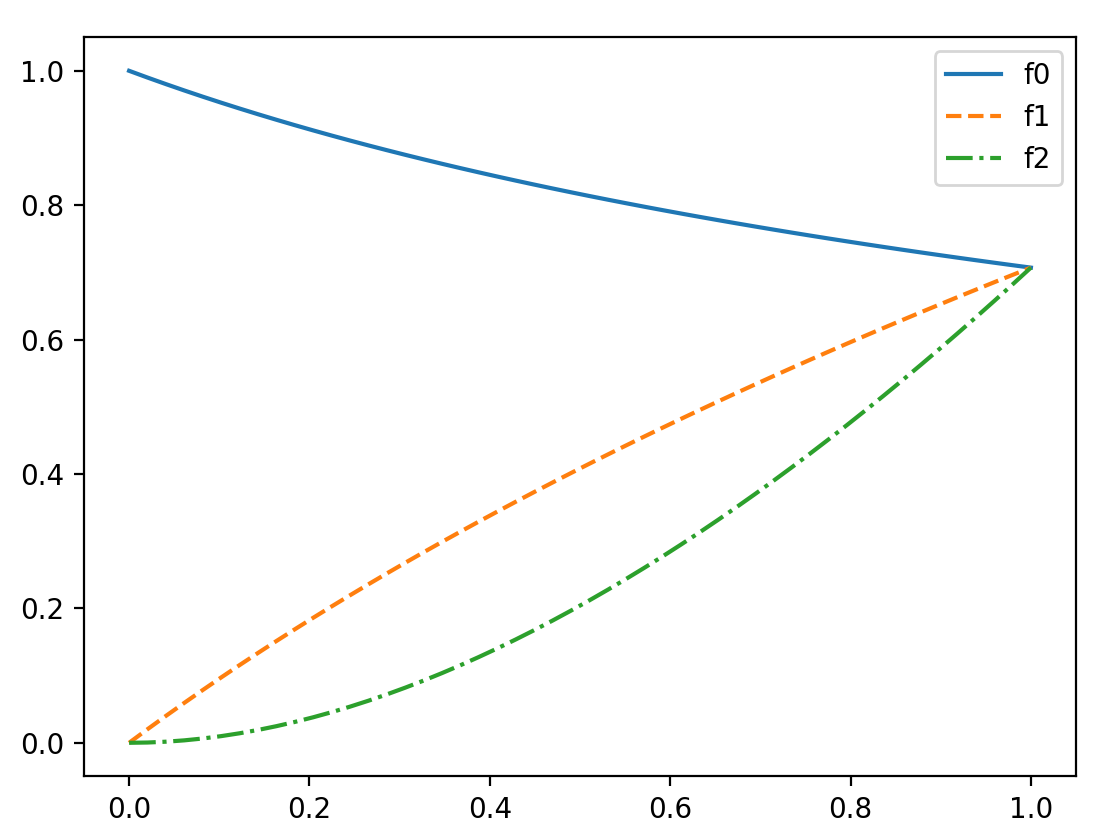
\includegraphics[scale=0.45]{DNS5c-fig}
  \end{center}
  \item Soit $x \in [0,1]$.
  \begin{itemize}
  \item Si $x=1$ alors pour tout entier $n \geq 0$,
  $$ f_n(x) = \dfrac{1}{\sqrt{2}}$$
  donc 
  $$ \lim_{n \rightarrow + \infty} f_n(x) = \dfrac{1}{\sqrt{2}}$$
  \item Si $x \in [0,1[$ alors :
  $$\lim_{n \rightarrow + \infty} f_n(x) = 0$$
  \end{itemize}
  Soit $f : [0,1] \rightarrow \mathbb{R}$ définie par :
  $$ f(x) = \left\lbrace \begin{array}{ccl}
  0 & \hbox{ si } x \in [0,1[ \\
  \dfrac{1}{\sqrt{2}} & \hbox{ si } x=1 \\
  \end{array}\right.$$
  Alors,
  \enc{$(f_n)_{n \geq 0}$ converge simplement sur $[0,1]$ vers $f$}
  \item \textit{Première méthode :} Supposons par l'absurde que $(f_n)_{n \geq 0}$ converge uniformément sur $[0,1]$ vers $f$. Pour tout $n \geq 0$, $f_n$ est continue sur $[0,1]$ donc $f$ est continue sur $[0,1]$ ce qui est absurde. 
  
  \medskip
  
   \textit{Deuxième méthode :} Pour tout entier $n \geq 1$, $f_n$ est continue sur le segment $[0,1]$ donc bornée sur celui-ci et cette fonction est croissante et positive donc :
  $$ \Vert f_n \Vert_{\infty} = f_n(1) = \dfrac{1}{\sqrt{2}}$$
  et cette constante est non nulle.
  
  \medskip
  
  On vient donc de montrer que 
  \enc{$(f_n)_{n \geq 0}$ ne converge pas uniformément sur $[0,1]$ vers $f$}
  \item 
  \begin{enumerate}
  \item Soit $n \geq 0$. Alors :
  \begin{align*}
  u_{n+1}-u_n & =  \int_0^1 f_{n+1}(x) \dx- \int_0^1 f_n(x) \dx \\
  & =  \int_0^1 f_{n+1}(x)-f_n(x) \dx
  \end{align*}
  par linéarité. On a pour tout $x \in [0,1]$,
  $$ f_{n+1}(x)-f_n(x) = \dfrac{x^{n+1}-x^n}{\sqrt{1+x}} = \dfrac{x^n(x-1)}{\sqrt{1+x}} \leq 0$$
  car $x \in [0,1]$. Par positivité de l'intégrale (les bornes sont dans le bon sens), on en déduit que :
  $$ u_{n+1}-u_n \leq 0$$
  Ainsi,
  \enc{$(u_n)_{n \geq 0}$ est décroissante}
  Pour étudier la convergence, encadrons l'intégrale (pas de convergence uniforme ici donc pas d'utilisation possible d'un théorème d'interversion). Soit $n \geq 0$. Pour tout $x \in [0,1]$, on a :
  $$ 1 \leq 1+x \leq 2$$
  donc par croissance de la fonction racine carré sur $\mathbb{R}_+$ :
  $$ 1 \leq \sqrt{1+x} \leq \sqrt{2}$$
  puis par décroissance de la fonction inverse sur $\mathbb{R}_+^{*}$ :
  $$ 1 \geq \dfrac{1}{\sqrt{1+x}} \geq \dfrac{1}{\sqrt{2}}$$
  Le réel $x^n$ est positif donc :
  $$ x^n \geq f_n(x) \geq \dfrac{x^n}{\sqrt{2}}$$
  Par croissance de l'intégrale (les bornes sont dans le bon sens), on en déduit que :
  $$ \int_0^1 x^n \dx \geq u_n \geq \dfrac{1}{\sqrt{2}} \int_0^1 x^n \dx$$
  et donc par simple calcul :
  $$ \dfrac{1}{n+1}\geq u_n \geq \dfrac{1}{\sqrt{2}}  \times\dfrac{1}{n+1}$$
  Sachant que :
  $$ \lim_{n \rightarrow + \infty} \dfrac{1}{n+1} =  \lim_{n \rightarrow + \infty}\dfrac{1}{\sqrt{2}}  \times\dfrac{1}{n+1} = 0$$
  On en déduit que $(u_n)_{n \geq 0}$ converge et que :
  \enc{$\lim_{n \rightarrow + \infty} u_n = 0$}
  \item Soit $n \geq 0$. On a :
  $$ (n+1)u_n = (n+1) \int_0^1 \dfrac{x^n}{\sqrt{1+x}} \dx = \int_0^1 (1+x)^{-1/2} \times (n+1) x^n \dx$$
  Les fonctions $x \mapsto (1+x)^{-1/2}$ et $x \mapsto x^{n+1}$ sont de classe $\mathcal{C}^1$ sur $[0,1]$, de dérivées respectives $x \mapsto (-1/2)(1+x)^{-3/2}$ et $x \mapsto (n+1)x^n$, donc par intégration par parties, on en déduit que :
  \begin{align*}
  (n+1) u_n & = \left[ \dfrac{x^{n+1}}{\sqrt{1+x}} \right]_0^1 + \dfrac{1}{2} \int_0^1 \dfrac{x^{n+1}}{(\sqrt{1+x})^3} \dx \\
  & = \dfrac{1}{\sqrt{2}}+ \dfrac{1}{2} \int_0^1 \dfrac{x^{n+1}}{(\sqrt{1+x})^3} \dx
  \end{align*}
  Ainsi, pour tout entier $n \geq 0$,
  $$ \boxed{(n+1) u_n = \dfrac{1}{\sqrt{2}} + \dfrac{1}{2} \int_0^1 \dfrac{x^{n+1}}{(\sqrt{1+x})^3} \dx}$$
  \item On montre, avec le même raisonnement que dans la question 5(a) (en utilisant que la fonction cube est croissante sur $\mathbb{R}$), que pour tout entier $n \geq 0$ et tout $x \in [0,1]$,
  $$ x^{n+1} \geq \dfrac{x^{n+1}}{(\sqrt{1+x})^3} \geq \dfrac{x^{n+1}}{\sqrt{2}^3}$$
  puis que :
  $$  \dfrac{1}{n+2} \geq \int_0^1 \dfrac{x^{n+1}}{(\sqrt{1+x})^3} \dx \geq \dfrac{1}{\sqrt{2}^3} \times \dfrac{1}{n+2}$$
  et finalement :
  $$ \lim_{n \rightarrow + \infty} \int_0^1 \dfrac{x^{n+1}}{(\sqrt{1+x})^3} \dx = 0$$
  On en déduit alors que :
  $$ \lim_{n \rightarrow + \infty} (n+1)u_n = \dfrac{1}{\sqrt{2}}=0$$
  et finalement,
  $$ \boxed{ u_n \underset{+ \infty}{\sim} \dfrac{1}{\sqrt{2}(n+1)} \underset{+ \infty}{\sim} \dfrac{1}{\sqrt{2}n} }$$
  \item On a pour tout entier $n \geq 0$,
  $$(n+1)(n+2) u_n = \dfrac{(n+2)}{\sqrt{2}} + \dfrac{n+2}{2} \int_0^1 \dfrac{x^{n+1}}{(\sqrt{1+x})^3} \dx$$
  %donc
  %$$ n u_n = - u_n + \dfrac{1}{\sqrt{2}} + \dfrac{1}{2} \int_0^1 \dfrac{x^{n+1}}{(\sqrt{1+x})^3} \dx$$
  %donc
  %$$ u_n = - \dfrac{u_n}{n} + \dfrac{1}{\sqrt{2} n } + \dfrac{1}{2n} \int_0^1 \dfrac{x^{n+1}}{(\sqrt{1+x})^3} \dx$$
  %puis
  %$$ u_n - \dfrac{1}{\sqrt{2} n } = - \dfrac{u_n}{n}  + \dfrac{1}{2n} \int_0^1 \dfrac{x^{n+1}}{(\sqrt{1+x})^3} \dx$$
  %Une intégration par parties bien justifiée montre que :
  %\begin{align*}
  % \int_0^1 \dfrac{x^{n+1}}{(\sqrt{1+x})^3} \dx & = \dfrac{1}{n+2} \left[ \dfrac{x^{n+2}}{(\sqrt{1+x})^3} \right]_0^1 + \dfrac{3}{2(n+2)} \int_0^1 \dfrac{x^{n+2}}{(\sqrt{1+x})^5} \dx \\
  %& = \dfrac{1}{(n+2)\sqrt{2}^3} + \dfrac{3}{2(n+2)} \int_0^1 \dfrac{x^{n+2}}{(\sqrt{1+x})^5} \dx 
  %\end{align*}
  
  
  %
  %
  %
  %$$ (n+2)(n+1)u_n =  \dfrac{n+2}{\sqrt{2}} + \dfrac{n+2}{2} \int_0^1 \dfrac{x^{n+1}}{(\sqrt{1+x})^3} \dx$$
  Une intégration par parties, bien justifiée, montre que :
  \begin{align*}
  (n+2) \int_0^1 \dfrac{x^{n+1}}{(\sqrt{1+x})^3} \dx & = \left[ \dfrac{x^{n+2}}{(\sqrt{1+x})^3} \right]_0^1 + \dfrac{3}{2} \int_0^1 \dfrac{x^{n+2}}{(\sqrt{1+x})^5} \dx \\
  & = \dfrac{1}{\sqrt{2}^3} + \dfrac{3}{2} \int_0^1 \dfrac{x^{n+2}}{(\sqrt{1+x})^5} \dx 
  \end{align*}
  On montre comme précédemment que :
  $$ \lim_{n \rightarrow + \infty} \dfrac{3}{2} \int_0^1 \dfrac{x^{n+2}}{(\sqrt{1+x})^5} \dx  = 0$$
  donc 
  $$ (n+2)(n+1)u_n \underset{+ \infty}{=}  \dfrac{n+2}{\sqrt{2}} + \dfrac{1}{2\sqrt{2}^3} + o(1) $$
  puis
  $$ u_n \underset{+ \infty}{=} \dfrac{1}{\sqrt{2}(n+1)}  +  \dfrac{1}{(n+2)(n+1)2\sqrt{2}^3} + o \left(\dfrac{1}{(n+2)(n+1)} \right)$$
  %Posons :
  %$$ \alpha = \sqrt{2} \; \hbox{ et } \; \beta = \dfrac{1}{2\sqrt{2}}$$
  %On a :
  %\begin{align*}
  %u_n - \dfrac{\alpha}{n} + \dfrac{\beta}{n^2} & \underset{+ \infty}{=} \dfrac{\sqrt{2}}{n+1} - \dfrac{\sqrt{2}}{n}  +  \dfrac{1}{(n+2)(n+1)2\sqrt{2}}- \dfrac{1}{2\sqrt{2}n^2} + o \left(\dfrac{1}{(n+2)(n+1)} \right)
  %\end{align*}
  On a :
  $$  \dfrac{1}{(n+2)(n+1)} \underset{+ \infty}{\sim} \dfrac{1}{n^2}$$
  donc 
  $$ \dfrac{1}{(n+2)(n+1)} \underset{+ \infty}{=} \dfrac{1}{n^2} + o \left( \dfrac{1}{n^2} \right)$$
  et on a aussi :
  \begin{align*}
  \dfrac{1}{n+1} & = \dfrac{1}{n} \left( \dfrac{1}{1+1/n} \right) \\
  &  \underset{+ \infty}{=}  \dfrac{1}{n} \left( 1- \dfrac{1}{n} + o \left( \dfrac{1}{n} \right) \right) \\
  & \underset{+ \infty}{=} \dfrac{1}{n} - \dfrac{1}{n^2} +  o \left( \dfrac{1}{n^2} \right)
  \end{align*}
  On a alors :
  \begin{align*}
  u_n & \underset{+ \infty}{=} \dfrac{1}{\sqrt{2}(n+1)}  +  \dfrac{1}{(n+2)(n+1)2\sqrt{2}^3} + o \left(\dfrac{1}{(n+2)(n+1)} \right) \\
  &  \underset{+ \infty}{=} \dfrac{1}{\sqrt{2}n} - \dfrac{1}{\sqrt{2} n^2}  + \dfrac{1}{4\sqrt{2}n^2}  +  o \left(\dfrac{1}{n^2} \right) \\
  %&  \underset{+ \infty}{=}\dfrac{1}{\sqrt{2}n}+ \left(- \sqrt{2} + \dfrac{1}{4\sqrt{2}} \right) \dfrac{1}{n^2} +  o \left(\dfrac{1}{n^2} \right) \\
  &  \underset{+ \infty}{=} \dfrac{1}{\sqrt{2}n} - \dfrac{3}{4\sqrt{2}} \times \dfrac{1}{n^2} +  o \left(\dfrac{1}{n^2} \right) 
  \end{align*}
  
  \end{enumerate}
  \end{enumerate}


\section*{Exercice 2}
  \begin{enumerate}
  \item Soit $x \in ]-1, + \infty[$. La suite $\left( \dfrac{1}{x+n} \right)_{n \geq 1}$ est positive, décroissante et converge vers $0$ donc d'après le critère spécial des séries alternées, la série de terme général $\dfrac{(-1)^n}{x+n}$ converge. Ainsi,
  \enc{$S$ est définie sur $I= ]-1, + \infty[$}
  \item Vérifions les hypothèse du théorème de continuité. Posons pour tout entier $n \geq 1$ et tout réel $x \in I$,
  $$ f_n(x) = \dfrac{(-1)^n}{x+n}$$
  et
  $$ R_n(x) = \sum_{k=n+1}^{+ \infty} f_k(x)$$
  Remarquons que $R_n(x)$ est bien défini car la série de terme général $f_k(x)$ converge.
  \begin{itemize}
  \item Pour tout entier $n \geq 1$, $f_n$ est continue sur $I$.
  \item D'après le critère spécial des séries alternées (hypothèses vérifiées dans la question précédente), on a pour tout $n \geq 1$ et tout $x \in I$,
  $$ \vert R_n(x) \vert \leq \left\vert \dfrac{(-1)^{n+1}}{x+n+1} \right\vert = \dfrac{1}{x+n+1} \leq \dfrac{1}{n}$$
  car $x>-1$. Ainsi, $R_n$ est bornée sur $I$ et :
  $$0 \leq \Vert R_n \Vert_{\infty} \leq \dfrac{1}{n}$$
  Or 
  $$ \lim_{n \rightarrow + \infty}  \dfrac{1}{n} = 0$$
  Par théorème d'encadrement, on en déduit que $\Vert R_n \Vert_{\infty}$ tend vers $0$ quand $n$ tend vers $+ \infty$ donc $(R_n)_{n \geq 1}$ converge uniformément vers la fonction nulle sur $I$ et ainsi, $\Sum{n \geq 1}{}f_n$ converge uniformément sur $I$.
  \end{itemize}
  Par théorème de continuité, on en déduit que 
  \enc{$S$ est continue sur $I$}
  \item Vérifions les hypothèses du dérivabilité.
  \begin{itemize}
  \item Pour tout entier $n \geq 1$, $f_n$ est de classe $\mathcal{C}^1$ sur $I$.
  \item $\Sum{n \geq 1}{}f_n$ converge simplement (car uniformément) sur $I$.
  \item Pour tout entier $n \geq 1$ et tout $x \in I$,
  $$ f_n'(x) =\dfrac{(-1)^{n+1}}{(x+n)^2}$$
  La suite de terme général $\dfrac{1}{(x+n)^2}$ est positive, décroissante et converge vers $0$ donc d'après le critère spécial des séries alternées, on en déduit que la série de terme général $f_n'(x)$ converge. En notant $T_n$ le reste d'ordre $n \geq 1$, on obtient comme dans la question précédente que $T_n$ est bornée sur $I$ et :
  $$ 0 \leq \Vert T_n \Vert_{\infty} \leq \dfrac{1}{n^2}$$
  Par théorème d'encadrement, on en déduit que $\Vert T_n \Vert_{\infty}$ tend vers $0$ quand $n$ tend vers $+ \infty$ donc $(T_n)_{n \geq 1}$ converge uniformément vers la fonction nulle sur $I$ et ainsi, $\Sum{n \geq 1}{}f_n'$ converge uniformément sur $I$.
  \end{itemize}
  Par théorème de dérivabilité, on en déduit que 
  \enc{$S$ est de classe $\mathcal{C}^1$ sur $I$}
  et pour tout $x \in I$,
  $$S'(x) = \sum_{n=1}^{+ \infty} \dfrac{(-1)^{n+1}}{(x+n)^2}$$
  D'après le critère spécial des séries alternées, $S'(x)$ est du signe de :
  $$ \dfrac{(-1)^{1+1}}{(x+1)^2} =  \dfrac{1}{(x+1)^2}>0$$
  Ainsi, $S'(x)$ est positif. On en déduit que 
  \enc{$S$ est croissante sur $I$}
  \item Vérifions les hypothèses du théorème d'interversion limite-somme :
  \begin{itemize}
  \item On a déjà montré que la série de fonctions de terme général $f_n$ converge uniformément sur $I$ (dont $+ \infty$ est une extrémité).
  \item Pour tout entier $n \geq 1$,
  $$ \lim_{x \rightarrow + \infty} \dfrac{(-1)^n}{x+n} = 0$$
  \end{itemize}
  D'après le théorème d'interversion limite-somme, on en déduit que $S$ admet une limite en $+ \infty$ et que celle-ci est nulle :
  $$ \boxed{\lim_{n \rightarrow + \infty} S(x) = 0}$$
  \item On souhaite utiliser le théorème d'interversion limite-somme mais la fonction $f_1$ n'a pas une limite finie en $-1^+$. On va \og oublier \fg cette fonction pour le moment.
  \begin{itemize}
  \item On sait que $\Sum{n \geq 1}{} f_n$ converge uniformément sur $I$ donc en particulier $\Sum{n \geq 2}{} f_n$ converge uniformément sur $I$.
  \item Pour tout entier $n \geq 2$,
  $$ \lim_{x \rightarrow -1^{+}} \dfrac{(-1)^n}{x+n} =  \dfrac{(-1)^n}{n-1}$$
  \end{itemize} 
  D'après le théorème d'interversion limite-somme, on en déduit que la fonction 
  $$ g: x \mapsto \sum_{n=2}^{+ \infty} \dfrac{(-1)^n}{x+n}$$
  admet une limite finie en $-1^{+}$ qui est égale à la somme de la série convergente de terme général $\dfrac{(-1)^n}{n-1}$ :
  $$ \lim_{x \rightarrow -1^+} g(x) = \sum_{n=2}^{+ \infty} \dfrac{(-1)^n}{n-1}$$
  Or, pour tout $x \in I$,
  $$ S(x) = \sum_{n=1}^{+ \infty} \dfrac{(-1)^n}{x+n} = - \dfrac{1}{x+1} + g(x)$$
  La fonction $g$ admet une limite finie en $-1^+$ et 
  $$ \lim_{x \rightarrow -1^+} -\dfrac{1}{x+1}=- \infty$$
  Par somme, on en déduit que :
  $$ \boxed{\lim_{x \rightarrow -1^+} S(x)= - \infty}$$
  
  \medskip
  
  \textit{Remarque}. On peut aussi utiliser le critère spécial qui montre que pour tout $n \geq 1$ et tout $x \in I$,
  $$ \vert R_1(x) \vert \leq \left\vert \dfrac{(-1)^2}{x+2} \right\vert = \dfrac{1}{x+2}$$
  et $R_1(x)$ est du signe de $\dfrac{(-1)^2}{x+2}$ donc positif ce qui implique que :
  $$ 0 \leq R_1(x) \leq \dfrac{1}{x+2}$$
  puis 
  $$ 0 \leq \sum_{n=2}^{+ \infty} \dfrac{(-1)^n}{x+n} \leq \dfrac{1}{x+2}$$
  et finalement 
  $$ - \dfrac{1}{x+1} \leq S(x) \leq \dfrac{1}{x+2} - \dfrac{1}{x+1}$$
  On conclut avec le théorème de comparaison en remarquant que :
  $$ \lim_{x \rightarrow -1^+} \dfrac{1}{x+2}-\dfrac{1}{x+1}=- \infty$$
  \end{enumerate}


\section*{Exercice 3}
\begin{itemize}
  \item Pour tout $n \geq 0$, $f_n$ est continue sur $\mathbb{R}$.
  \item Pour tout $n \geq 0$ et tout $x \in \mathbb{R}$,
  $$ \vert f_n(x) \vert \leq \vert a_n \vert = a_n$$
  car $a_n \geq 0$. Ainsi, $f_n$ est bornée sur $\mathbb{R}$ et 
  $$ 0 \leq \Vert f_n \Vert_{\infty} \leq a_n$$
  La série de terme général positif $a_n$ converge donc par critère de comparaison, la série de terme général $\Vert f_n \Vert_{\infty}$ converge donc la série de fonctions de terme général $f_n$ converge normalement (donc uniformément) sur $\mathbb{R}$.
  \end{itemize}
  Par théorème de continuité, on en déduit que :
  \enc{$f$ est bien définie et continue sur $\mathbb{R}$}
  
  \medskip
  
  Vérifions les hypothèses du théorème de dérivabilité (on donnera une condition simple au moment où on en a besoin).
  
  \begin{itemize}
  \item La série de fonctions de terme général $f_n$ converge simplement sur $\mathbb{R}$ (car uniformément d'après le raisonnement précédent).
  \item Pour tout $n \geq 0$, $f_n$ est de classe $\mathcal{C}^1$ et :
  $$ \forall x \in \mathbb{R}, \; f_n'(x) = -n a_n \sin(nx)$$
  \item Pour tout $n \geq 0$ et tout $x \in \mathbb{R}$,
  $$ \vert f_n'(x) \vert \leq \vert n a_n \vert = n a_n$$
  car $a_n \geq 0$. Ainsi, $f_n$ est bornée sur $\mathbb{R}$ et 
  $$ 0 \leq \Vert f_n' \Vert_{\infty} \leq n a_n$$
  Sous la condition que la série de terme général positif $n a_n$ converge, on en déduit par critère de comparaison des séries à termes positifs que la série de terme général $\Vert f_n' \Vert_{\infty}$ converge donc la série de fonctions de terme général $f_n'$ converge normalement (donc uniformément) sur $\mathbb{R}$.
  \end{itemize}
  Par théorème de dérivabilité, on en déduit que :
  \enc{$f$ est de classe $\mathcal{C}^1$ sur $\mathbb{R}$}


\end{document}